\documentclass[10pt]{article}
\usepackage[a4paper,margin=0.85in]{geometry}
\usepackage{graphicx}
\usepackage{booktabs}
\usepackage{amsmath,amssymb}
\usepackage{xcolor}
\usepackage[colorlinks=true,linkcolor=blue,urlcolor=blue]{hyperref}
\usepackage{titlesec}
\titlespacing*{\section}{0pt}{6pt}{3pt}
\titlespacing*{\subsection}{0pt}{5pt}{2pt}
\setlength{\parskip}{2pt}
\setlength{\parindent}{0pt}

\title{\vspace{-1.4cm}\textbf{CS771: Intro to Machine Learning, Mini-Project 1}}
\author{Vedant Tiwari (221184)}
\date{}

\begin{document}
\maketitle
\vspace{-0.6cm}

\section{Introduction}
We are given three binary-classification datasets that encode the same inputs under three different
feature representations: 13 emoticons per input, a $13\times768$ deep-feature embedding matrix, and a
50-digit string. The train, validation, and test splits have $7080$, $489$, and $2232$ examples and are
almost perfectly class-balanced ($3576$ vs.\ $3504$). I checked that the label ordering is the same across
the three representations, which is what lets us combine them at the decision level in Task~2. Every model
below stays within the 10{,}000 trainable-parameter budget; for a linear model this is (number of features
$+\,1$ bias).

\section{Dataset analysis}
\textbf{Emoticon.} Each input has exactly 13 emojis drawn from a vocabulary of 214. Seven emojis occur in
every row (four of them once and three of them twice), which fills 10 of the 13 slots, so only 3 slots carry
``content'' emojis (207 distinct ones). A bag-of-content-emojis model sits at chance ($\sim$52\%), while a
positional one-hot encoding reaches 91\%. So the label depends on where the tokens sit, not just on which
content emojis are present.

\textbf{Deep features.} A $13\times768$ float matrix per input, roughly zero-mean with values in
$[-0.93,0.87]$. Averaging the 13 embeddings into one vector drops accuracy to about 50\%, because the
average throws away the position of each embedding, so I keep the positions instead.

\textbf{Text sequence.} Digit strings of length 44 to 47. Short substrings repeat with a fixed multiplicity
(\texttt{15436} appears once in every row, \texttt{1596} about twice), so the string looks like a
concatenation of one code per emoji, with the padding emojis giving constant codes. The code lengths vary
and their offsets shift from row to row, so splitting a string cleanly back into 13 ordered codes is
ambiguous, and the rules do not allow using the other two datasets to decode it. This is why the sequence
is the hardest of the three.

\section{Task 1: one model per dataset}
For each dataset I used linear models (Logistic Regression or a linear SVM). With a 10k-parameter cap a
linear model on a good feature map is both the natural choice and, in practice, the ceiling: even one small
hidden layer over the $\sim$2{,}800 one-hot features would exceed the budget. The regularisation strength
$C$ was tuned on the validation set. Table~\ref{tab:t1} lists the final choices.

\begin{table}[h]
\centering\small
\begin{tabular}{@{}llrr@{}}
\toprule
Dataset & Final model (features, then classifier) & Params & Val.\ acc. \\
\midrule
Emoticon & positional one-hot $(13{\times}214)$, LogReg $C{=}5$ & 2{,}783 & 91.00\% \\
Deep features & flatten $(13{\times}768{=}9984)$, LogReg $C{=}0.3$ & 9{,}985 & 98.57\% \\
Text sequence & pos.\ one-hot $(500)$ + char $n$-gram counts $(9000)$, LogReg $C{=}1$ & 9{,}501 & 76.89\% \\
\bottomrule
\end{tabular}
\caption{Best model per dataset. Params counts trainable weights plus bias.}
\label{tab:t1}
\end{table}

For the emoticon data, the positional one-hot encodes each (slot, emoji) pair, so it captures the
arrangement that the label actually depends on; a plain bag of emojis and adding content-emoji bigrams both
failed to help. For the deep features, flattening keeps the positional structure and, at 9984 features,
stays under the budget, whereas mean-pooling and PCA both collapsed. For the sequence, positional digit
one-hot on its own reached about 66\%; adding character $n$-gram $(2\text{ to }5)$ counts, which pick up
code adjacency, raised it to about 77\% while staying under 10k parameters.

Figure~\ref{fig:t1} shows validation accuracy when only the first $\{20,40,60,80,100\}\%$ of the training
data is used. The deep features are very data-efficient and already reach 96.7\% with a fifth of the data,
while the emoticon and especially the sequence models keep improving as more data is added, which suggests
they carry a weaker and harder-to-learn signal.

\begin{figure}[h]
\centering
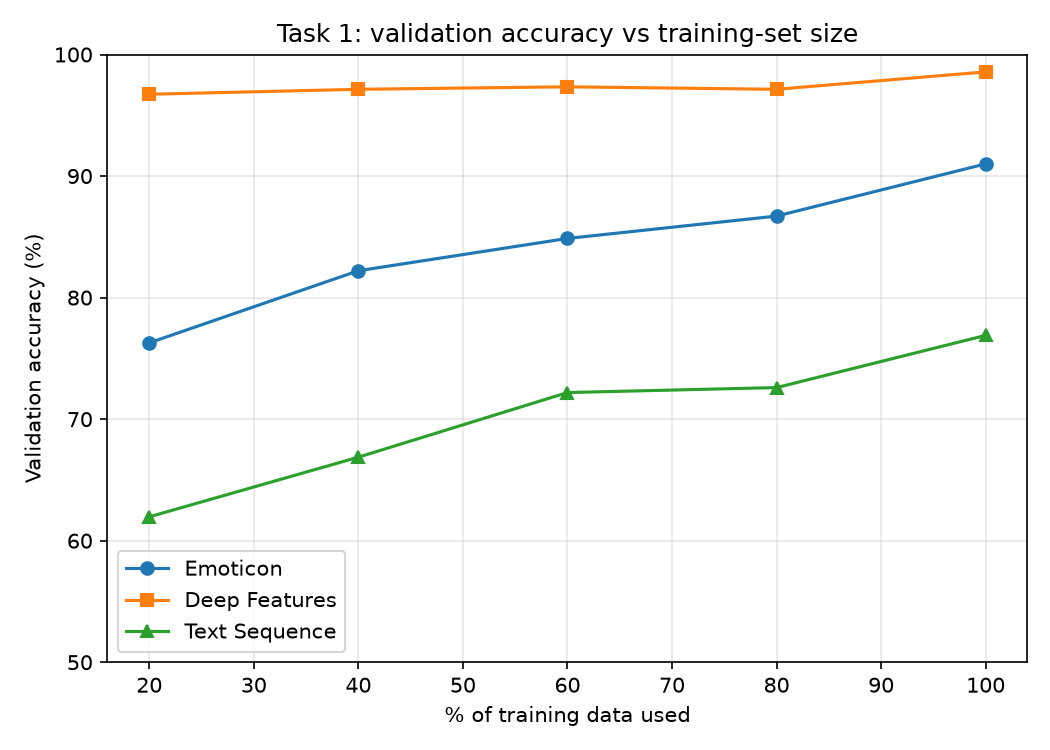
\includegraphics[width=0.6\textwidth]{plots/task1_sweep.png}
\caption{Validation accuracy against training-set size for the three datasets.}
\label{fig:t1}
\end{figure}

\section{Task 2: combining the three datasets}
Because the three views share their labels row for row, I combined them at the decision level with stacking.
Each base model outputs $P(y{=}1)$, and a logistic meta-model (3 inputs plus a bias, so 4 trainable
parameters) is trained on 5-fold out-of-fold base probabilities to avoid leakage. I also tried plain and
accuracy-weighted soft voting.

\begin{table}[h]
\centering\small
\begin{tabular}{@{}lccccc@{}}
\toprule
Combining method & 20\% & 40\% & 60\% & 80\% & 100\% \\
\midrule
Soft vote (mean probability) & 87.12 & 90.18 & 91.62 & 92.64 & 94.48 \\
Weighted soft vote & 88.96 & 92.23 & 94.07 & 93.87 & 95.71 \\
Stacking (logistic meta-model) & 96.73 & 96.93 & 97.34 & 97.14 & 98.57 \\
\bottomrule
\end{tabular}
\caption{Validation accuracy of the combination strategies against training-set size.}
\label{tab:t2}
\end{table}

Stacking matches the deep-features model at 98.57\% but does not improve on it. The meta-model weights are
about $(-0.07,\,12.1,\,0.10)$ for (emoticon, deep, sequence), so it puts almost all of the weight on the
deep view. That is consistent with the deep embeddings already capturing most of the recoverable signal,
which leaves little for the weaker emoticon and sequence views to add. Plain soft voting is in fact worse,
at 94.5\%, because the weak sequence model pulls the average down. My best model is therefore the single
deep-features classifier, and combining the datasets does not beat it. The reason seems to be redundancy
between the representations rather than a problem with the combiner.

\begin{figure}[h]
\centering
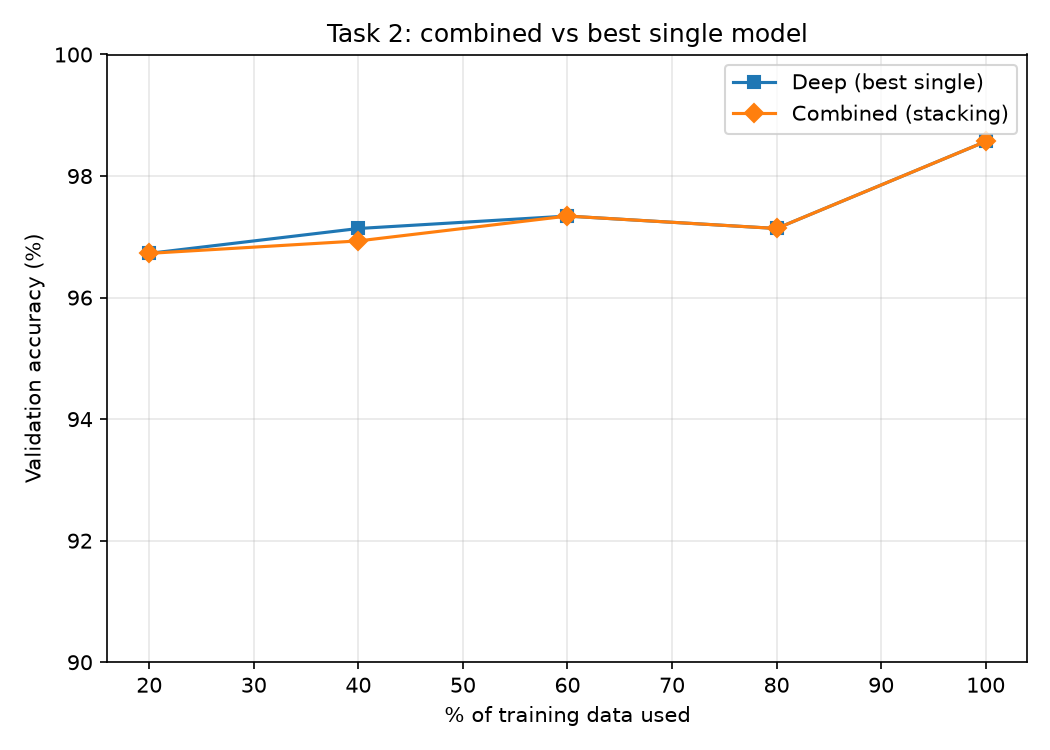
\includegraphics[width=0.56\textwidth]{plots/task2_sweep.png}
\caption{Stacking recovers the best single model but does not exceed it.}
\label{fig:t2}
\end{figure}

\section{Summary}
The emoticon model (positional one-hot with Logistic Regression) reaches 91.0\% with 2{,}783 parameters.
The deep-features model (flatten with Logistic Regression) reaches 98.57\% with 9{,}985 parameters and is
the best overall. The text-sequence model (positional one-hot plus character $n$-grams with Logistic
Regression) reaches 76.89\% with 9{,}501 parameters. The combined model (out-of-fold stacking) reaches
98.57\% and gives no gain over the deep features alone. All models stay within the 10{,}000-parameter
budget. The script \texttt{main.py} retrains every model from scratch with fixed seeds in under 20 seconds
and writes the four prediction files. The only libraries used are NumPy, pandas, and scikit-learn, and no
pre-trained feature extractor is used beyond the provided deep features.

\end{document}
